\listfiles
\documentclass[acmtog, review, screen]{acmart}
%\setcitestyle{super,sort&compress}
\citestyle{acmauthoryear}
\usepackage{booktabs} % For formal tables
\usepackage{graphicx}
\usepackage[ruled]{algorithm2e} % For algorithms

% Metadata Information
\acmYear{2018}
\acmMonth{1}

%\acmBadgeL[http://ctuning.org/ae/ppopp2016.html]{ae-logo}
%\acmBadgeR[http://ctuning.org/ae/ppopp2016.html]{ae-logo}

% Copyright
\setcopyright{acmcopyright}
%\setcopyright{acmlicensed}
%\setcopyright{rightsretained}
%\setcopyright{usgov}
%\setcopyright{usgovmixed}
%\setcopyright{cagov}
%\setcopyright{cagovmixed}

% DOI

\begin{document}

% Title portion
\title{Sentiment of the Union}
 \subtitle{Sentiment Analysis on Presidential State of the Union Addresses}
 
\author{Chase Rydeen}
\affiliation{%
  \institution{University of Mississippi}
  \streetaddress{1 University Dr}
  \city{University}
  \state{MS}
  \postcode{38677}
  \country{USA}}
\email{dcrydeen@go.olemiss.edu}

\begin{abstract}
As the machine learning and data science craze sweeps the nation, the implications and implementations are vast.
This paper takes a look at both of them through the lens of a topic of national importance, at the very least for the United States.
This topic is the words used by past Presidents of the United States, which are being pulled from their State of the Union Addresses.
These two broad subjects are implemented in varying degree by means of Natural Language Processing (NLP), of which this paper is centered around.
Natural Language Processing pulls heavily from both of these two categories to enable effective analysis of text-based data.
Using NLP, a sentiment analysis was conducted on the Addresses to gain further insight into the tone used by Presidents over the course of history.
This paper shares the methodology used to conduct this sentiment analysis and discusses how it was presented and \href{https://turing.cs.olemiss.edu/~dcrydeen/thesis/index.html}{visualized}.
\end{abstract}

\maketitle

\section{Introduction}
The words that we as humans speak have an incredible amount of weight behind them.
As the main form of communication in our society, words are ever more important for how we convey our ideas and our thoughts.
Words are crucial in how we communicate to others and no other person's word carries more meaning and power than the President of the United States.
The President of the United States is the leader of the free world and what he says shapes the identity of the United States and also much of the Western world.
Each President's words can provide great insight into the current state of the country and the world at large.
Depending on the tone, context, verbiage, and many other linguistic signals, one can interpret what is being said beyond the words actually being used.
While this is a daunting task programmatically, there are interesting patterns that can be identified by just analyzing the words themselves.
The analysis of Presidential State of the Union Addresses forms the basis for this thesis. 
The goal of this research is to examine the deeper meaning behind these speeches to gain greater insight into the status of the United States and the world at large at the time the address was delivered. 
The central question here being: can one use the words a President is speaking to accurately predict his position on the political spectrum, as well as predict how his speech is impacted by the current events at the time.

\section{Tools}
This research centers around Natural Language Processing (NLP) of textual data.
The NLTK, Natural Language Toolkit, which is a useful set of tools that implement many Natural Language Processing tasks, was used to develop the code needed to process the texts.
Research for the thesis was collected from various sources across the web that analyze the Presidential addresses from a historical perspective rather than a linguistic one.
One of the central goals of this thesis was to determine if Natural Language Processing techniques can be used successfully to learn trends in speech and etymology to make predictions about the people making those speeches.

\subsection{NLP and NLTK}
The Natural Language ToolKit provides a library of NLP methods to process text and extract meaningful trends and patterns from the text of interest.
The NLTK is implemented using Python, which is a simple, yet powerful language with excellent functionality for processing linguistic data \cite{nltk}.

\subsection{State of the Union Addresses}
The focus of this research centers around the State of the Union (SOTU) addresses, but the methods could be applied to other corpora as well.
These annual SOTU addresses allow the President to opine the issues of the time and also shape the narrative for the entire country.
The consistent collection of this text data makes it a good corpus to examine and it is very relevant to all United States citizens.
Also, because these addresses are heavily examined and discussed, more meaningful observations can be made about them.
And finally, because the political figures giving these speeches have such a public persona with many speeches and quotes on the record, it should be possible to categorize their speech patterns and use them as a basis for comparison and to make accurate predictions concerning the President's speech patterns and political leaning.

\subsection{D3.js}
D3.js (D3) is a JavaScript library for manipulating documents based on data. 
D3 helps bring data to life using HTML, SVG, and CSS. 
D3's emphasis on web standards gives you the full capabilities of modern browsers without being tied to a proprietary framework, combining powerful visualization components and a data-driven approach to DOM manipulation \cite{d3}.
D3 was used to create the visualizations on the web interface displaying the plots of the sentiment analysis for each president.
D3 is an effective tool for implementing interaction in visualizations and allows for greater understanding of the data being displayed.

\section{Preprocessing}
There are a great many intricacies when it comes to dealing with text data.
As such, there was a lot of preprocessing that had to be done in order to morph the data into a cleaner data set to extract the sentiment.
The main preprocessing hurdles were how to construct the lexicon, how to split out the categories of the lexicon, and how to handle certain speech and language phenomenon.

\subsection{Lexicon Approaches}
The first obstacle was how to develop and implement the lexicon.
The strength of the sentiment analysis is only as strong as the lexicon it is built upon, so this was an important task to get right.

\subsubsection{Objective Content-based Lexicon}
The first attempt made dumped all of the unique words out of the entirety of all the addresses, and then a manual sentiment score was assigned to each word to try and output a score for each address.
This implementation was not very effective as the manual assignment of scores was flawed and not very informed, so the sentiment scores produced were erratic and did not seem to show any pattern.
An objective dictionary of terms is hard to create without a lot of input since an individual's perception of certain words can be biased so it is better to crowd-source such efforts, as was done in approach 2.

\subsubsection{Objective Crowd-Sourced Lexicon}
The second attempt to create a lexicon used an already existing lexicon and fitted it for the purpose here.
This lexicon was developed using thousands of respondents and having them each rate a certain set of words and then each one of these responses was averaged into that word's sentiment score.
The lexicon has 8072 words in it used to score each one of the addresses, but there were some additional obstacles that had to be overcome in handling the words in order to successfully analyze them \cite{lexicon}.

\subsection{Intricacies}
The subtleties in speech and language make for some interesting problems when it comes to processing text data.
Much of natural language is spoken in phrases so these had to be caught and handled in order to derive their full meaning from the text on the page.
An important topic to discuss here are n-grams, a way to deal with these phrases.
N-grams link words together in phrases and enables a sentiment score for an entire phrase versus just a single word \cite{nltk}.
The biggest hurdles when it comes to phrases were negation and intensifiers, and for individual words was stemming.

\subsubsection{Handling Negation}
One of the most important facets of spoken language to address is negation.
People use negation in their lives frequently to turn a "good" into a "not bad".
Simple natural language processing algorithms work by splicing each word into a different index of an array and then compare the sentiment score for each word and get a total score.
So in this scenario it would ignore "not" as it would be considered an article and then would assign a moderately negative value to bad when it should have assigned a moderately positive value \cite{sentimentanalysis}.
There are multiple solutions to this problem involving the use of bigrams and linking the score from a phrase to both words [Bigrams], or do the correction in the actual processing portion of the scores.
The latter path was chosen, and in handling negation, if a word was preceded by a negation word (no, not, never), then its count was decrease by one (same effect as adding a negated term to the total).
The solution was a simple one, and might not have been as effective as other possible solutions with a more fine-tuned value approximation given the strength of the negation, which will be addressed in the future.

\subsubsection{Handling Intensifiers}
One of the next tasks to tackle was handling of intensifiers in the text.
The exact problem here was how to quantify an intensifier in the text so as to give more weight to "very hard" than to "hard".
Again, a simple solution was chosen here in that an "intensifier counter" kept track of the number of intensifiers preceding each word in the text.
Then, in the processing portion of the sentiment analysis, the total count of intensifiers is taken and that number of scores is multiplied by two, and the rest of the scores is treated normally.
For example, if the word is sad and it was spoken 24 times and had an intensifier count of 8 and a sentiment score of -.6, then 8 of those values were doubled to -1.2, and the rest were kept at -.6, and then the scores were added up as normal for that specific number.
The glaring fault here is that no two intensifiers are the same as "very" and "extremely" have two very different intensifying effects but that can be improved upon in the future.
The foundation for the intensifier system has been laid and the specifics can be tweaked to make the algorithm more specific, insomuch as can be achieved, given the subjective nature of the intensifiers and language in general.

\subsubsection{Handling Stemming}
The third and final major hurdle was that of stemming.
The lexicon that was used to classify and score the words was limited in scope.
Even though the 8000 word count of the lexicon used seems vast, it is by no means a comprehensive list of all words to be considered.
As a result of this limited lexicon, some words that have slightly different endings were glossed over and not counted correctly.
In order to solve this problem, an effective stemming method had to be found that would accommodate the most words and account for the words that were being missed.
The solution here was relatively simple as well, each word is taken and if there is not a match to a lexicon word then the word is stemmed by cutting off the last letter and comparing it to the lexicon again and looking for a match.
This process is done for each of the last three letters of any word, long enough to account for most ending changes and also not giving false positives for simpler common words.
The other alternative here would be a lemmatization algorithm that would try to simplify each word in meaning to a simpler word and compare that to the lexicon \cite{stem}.
This approach would have added a lot more overhead with a potentially marginal increase in lexicon matching, so in order to retain the relative speed of the current algorithm, a more simple approach was taken described above.

\subsection{Lexicon Categories}
After the main algorithm was created and processed, a sentiment score for each president was recorded for their tone in their presidential address.
The results here were interesting but did not say as much as they potentially could, so an additional layer was added to the algorithm to hopefully add more depth to it.
This addition was to add topic categories to the algorithm and produce a sentiment score for each president for each one of the categories as well as an overall score for the entire SOTU address.
The categories that were added were: Crime, Economy, Education, Energy, Environment, Family, Foreign Affairs, Government, Jobs, Religion, Terrorism, and War.
A text file was created for each one of these categories containing keywords pertaining to the topic of each one, which was constructed by choosing 5 different addresses from all of the addresses and reading them through and constructing the files based on the most commonly used words when referring to a certain sector of the United States.
An additional step was then added to the preprocessing portion of the algorithm where each sentence was scanned for any of the keywords and if it contained one then it was added to an array of sentences pertaining to that category.
After the entire address has been processed then a sentiment score is computed for the overall address, as well as the individual categories to get each president's tone pertaining to certain categories relevant to the United States at the time.

\begin{algorithm}[t]
\SetAlgoNoLine
\KwIn{All State of the Union Addresses}
\KwOut{The sentiment score for each Presidential Address for each category.}
open all .txt files and store them in lists of special category trigger words\;
\For{each address in the State of the Union Addresses}
	{format address
	split address in to sentences
	\For{each sentence in the address}
		{add sentence to 'overall' category
		\If{sentence contains category trigger word}
		{add sentence to category}
	\For{each category}
		{append list of sentences for that category to an overall list}
	\For{each topic in the overall list}
		{\For{each word in the topic}
			{create word count for each word and store it in a dictionary\;
			\If{previous word negator}
				{increment negator counter for that word by one}
			\If{previous word intensifier}
				{increment intensifier counter for that word by one}
			}
		\For{each word in the dictionary}
		{\If{word is in lexicon}
		{\If{length of negators[word] != 0}
		{Subtract length from total count for that word}
		}
		\If{length of intensifiers[word] != 0}
		{Raise length number of scores to the power of 2}
		Calculate the Sentiment Score by multiplying the number of occurences of the term by the score in the lexicon.
		}
		}
	}
	}
	
\caption{Sentiment Analysis Algorithm}
\label{alg:one}
\end{algorithm}

\section{Visualization}
Once the data was processed, an effective means for communicating the data had to be chosen.
Since one of the axes for the data here was the date on which the SOTU address was given, the first visualization is that of a line plot, showing the sentiment score for each address over time.
A second visualization was chosen to complement these scores and that is a word cloud.
A word cloud is a short visual summary of the most frequently used words in a body of text, with the respective word size indicating the frequency with which that term was used.

\subsection{Line Plot}
\begin{figure}
  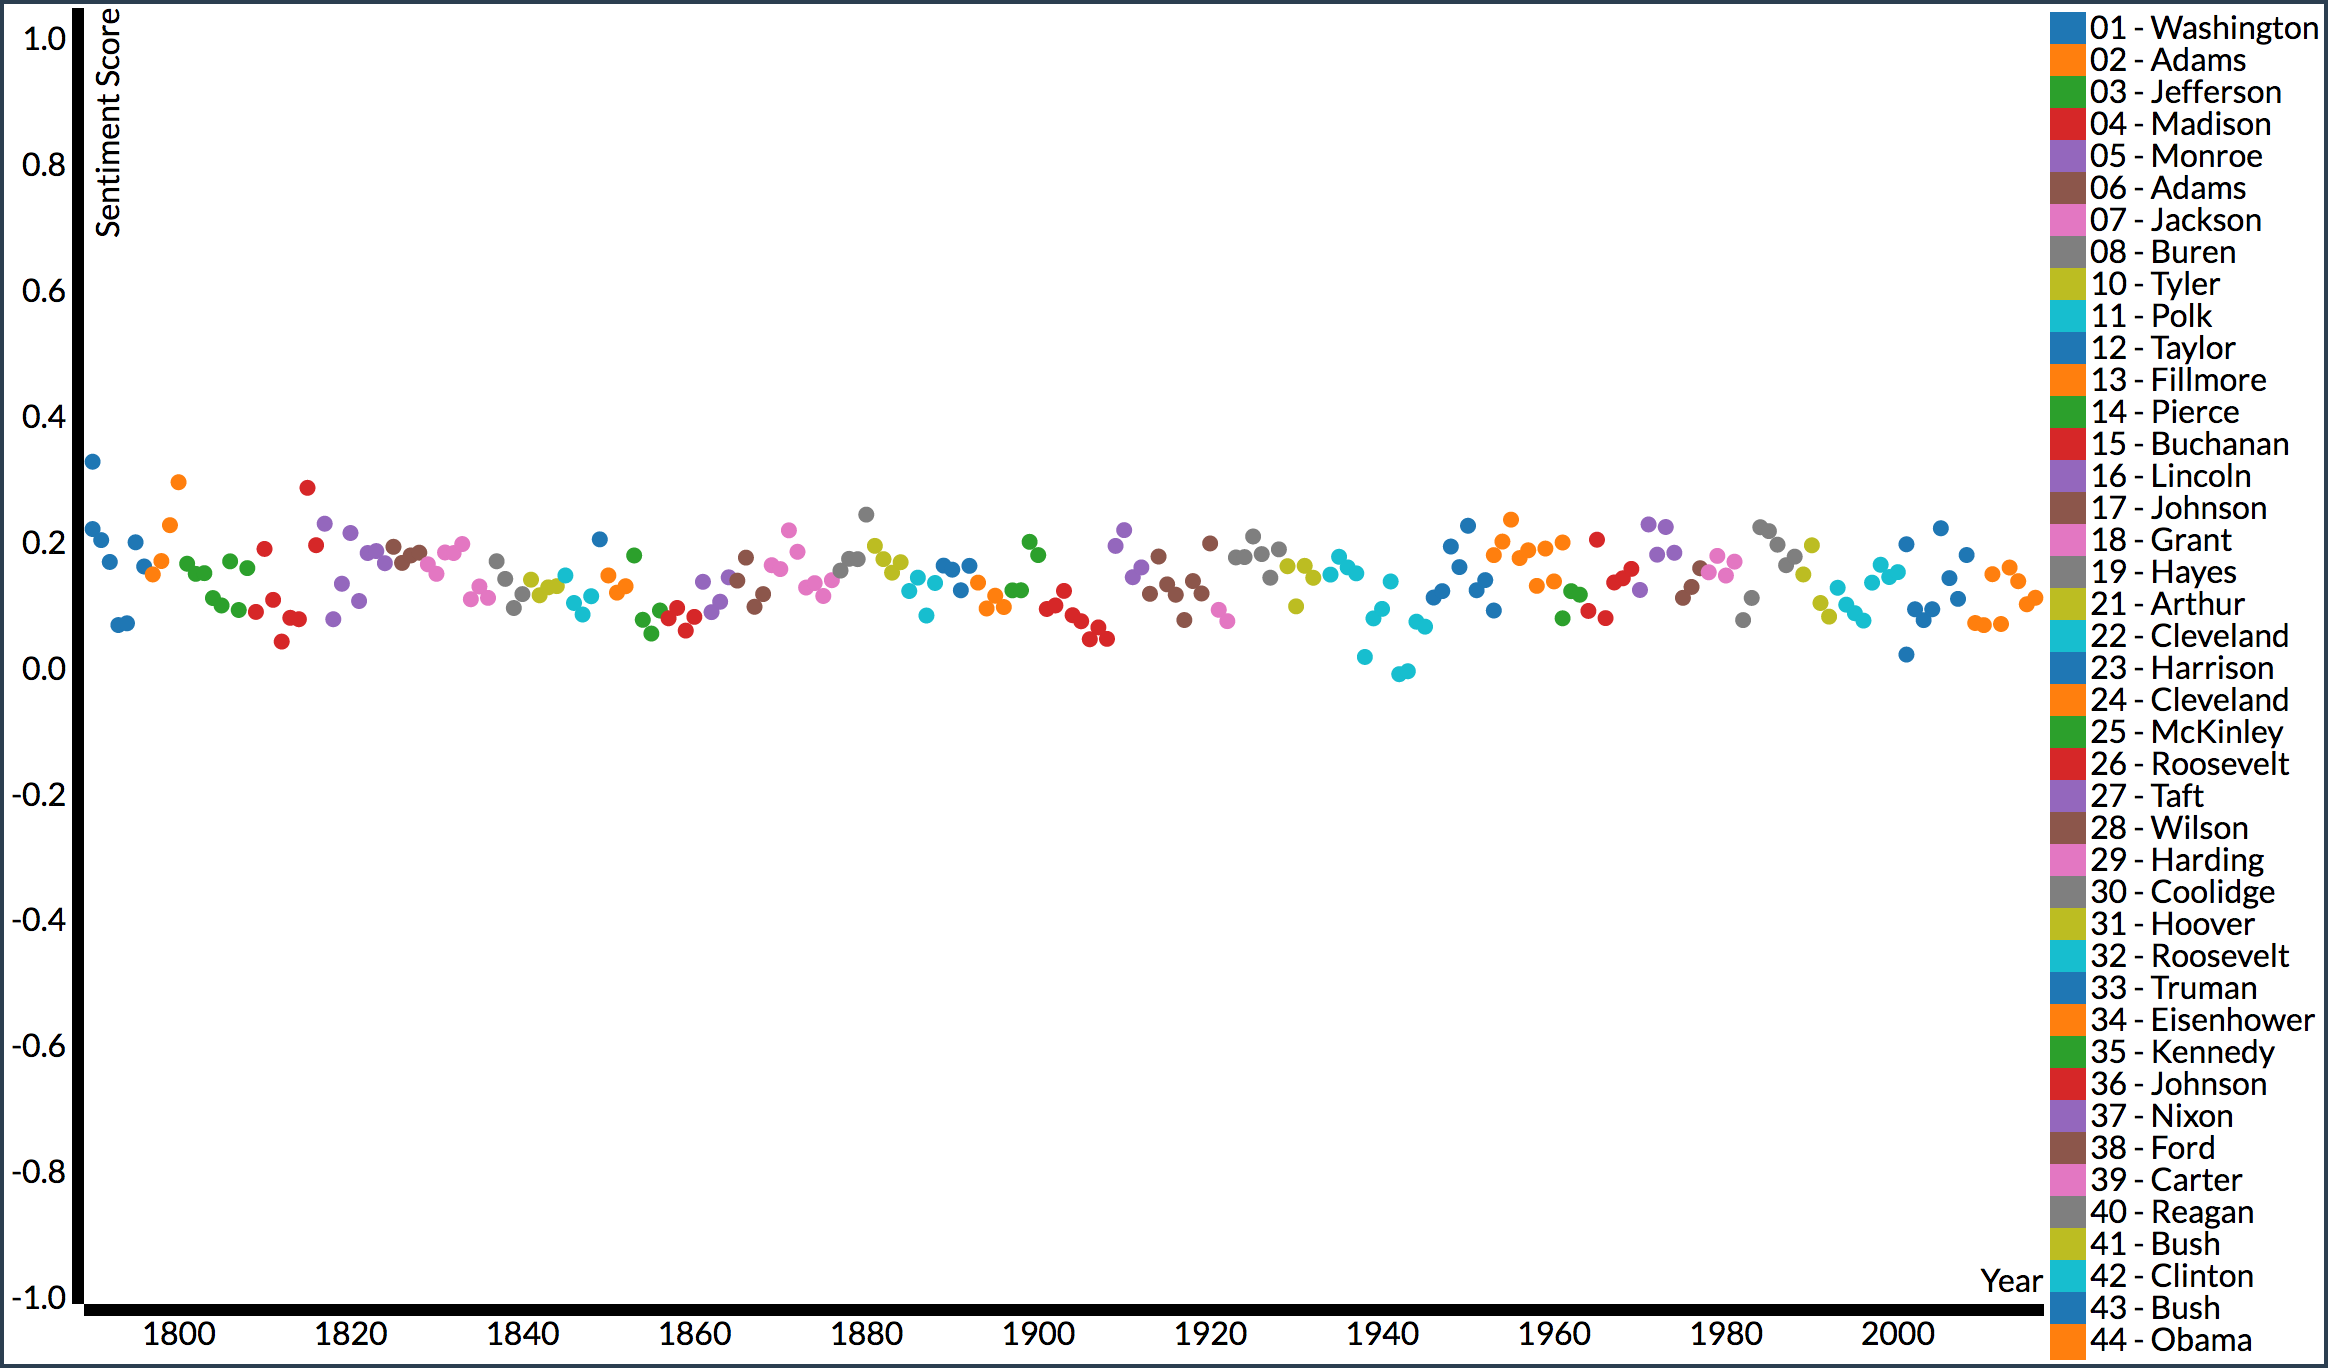
\includegraphics[width=\columnwidth]{Lineplot.png}
  \caption{Line Plot}
  \label{fig:lineplot1}
\end{figure}
The line plot constructed here shows all of the SOTU address sentiment scores plotted over time.
They are color-coded by president and the legend on the right shows each of the presidents and their respective color as can be seen in Figure \ref{fig:lineplot1}.
\begin{figure}
  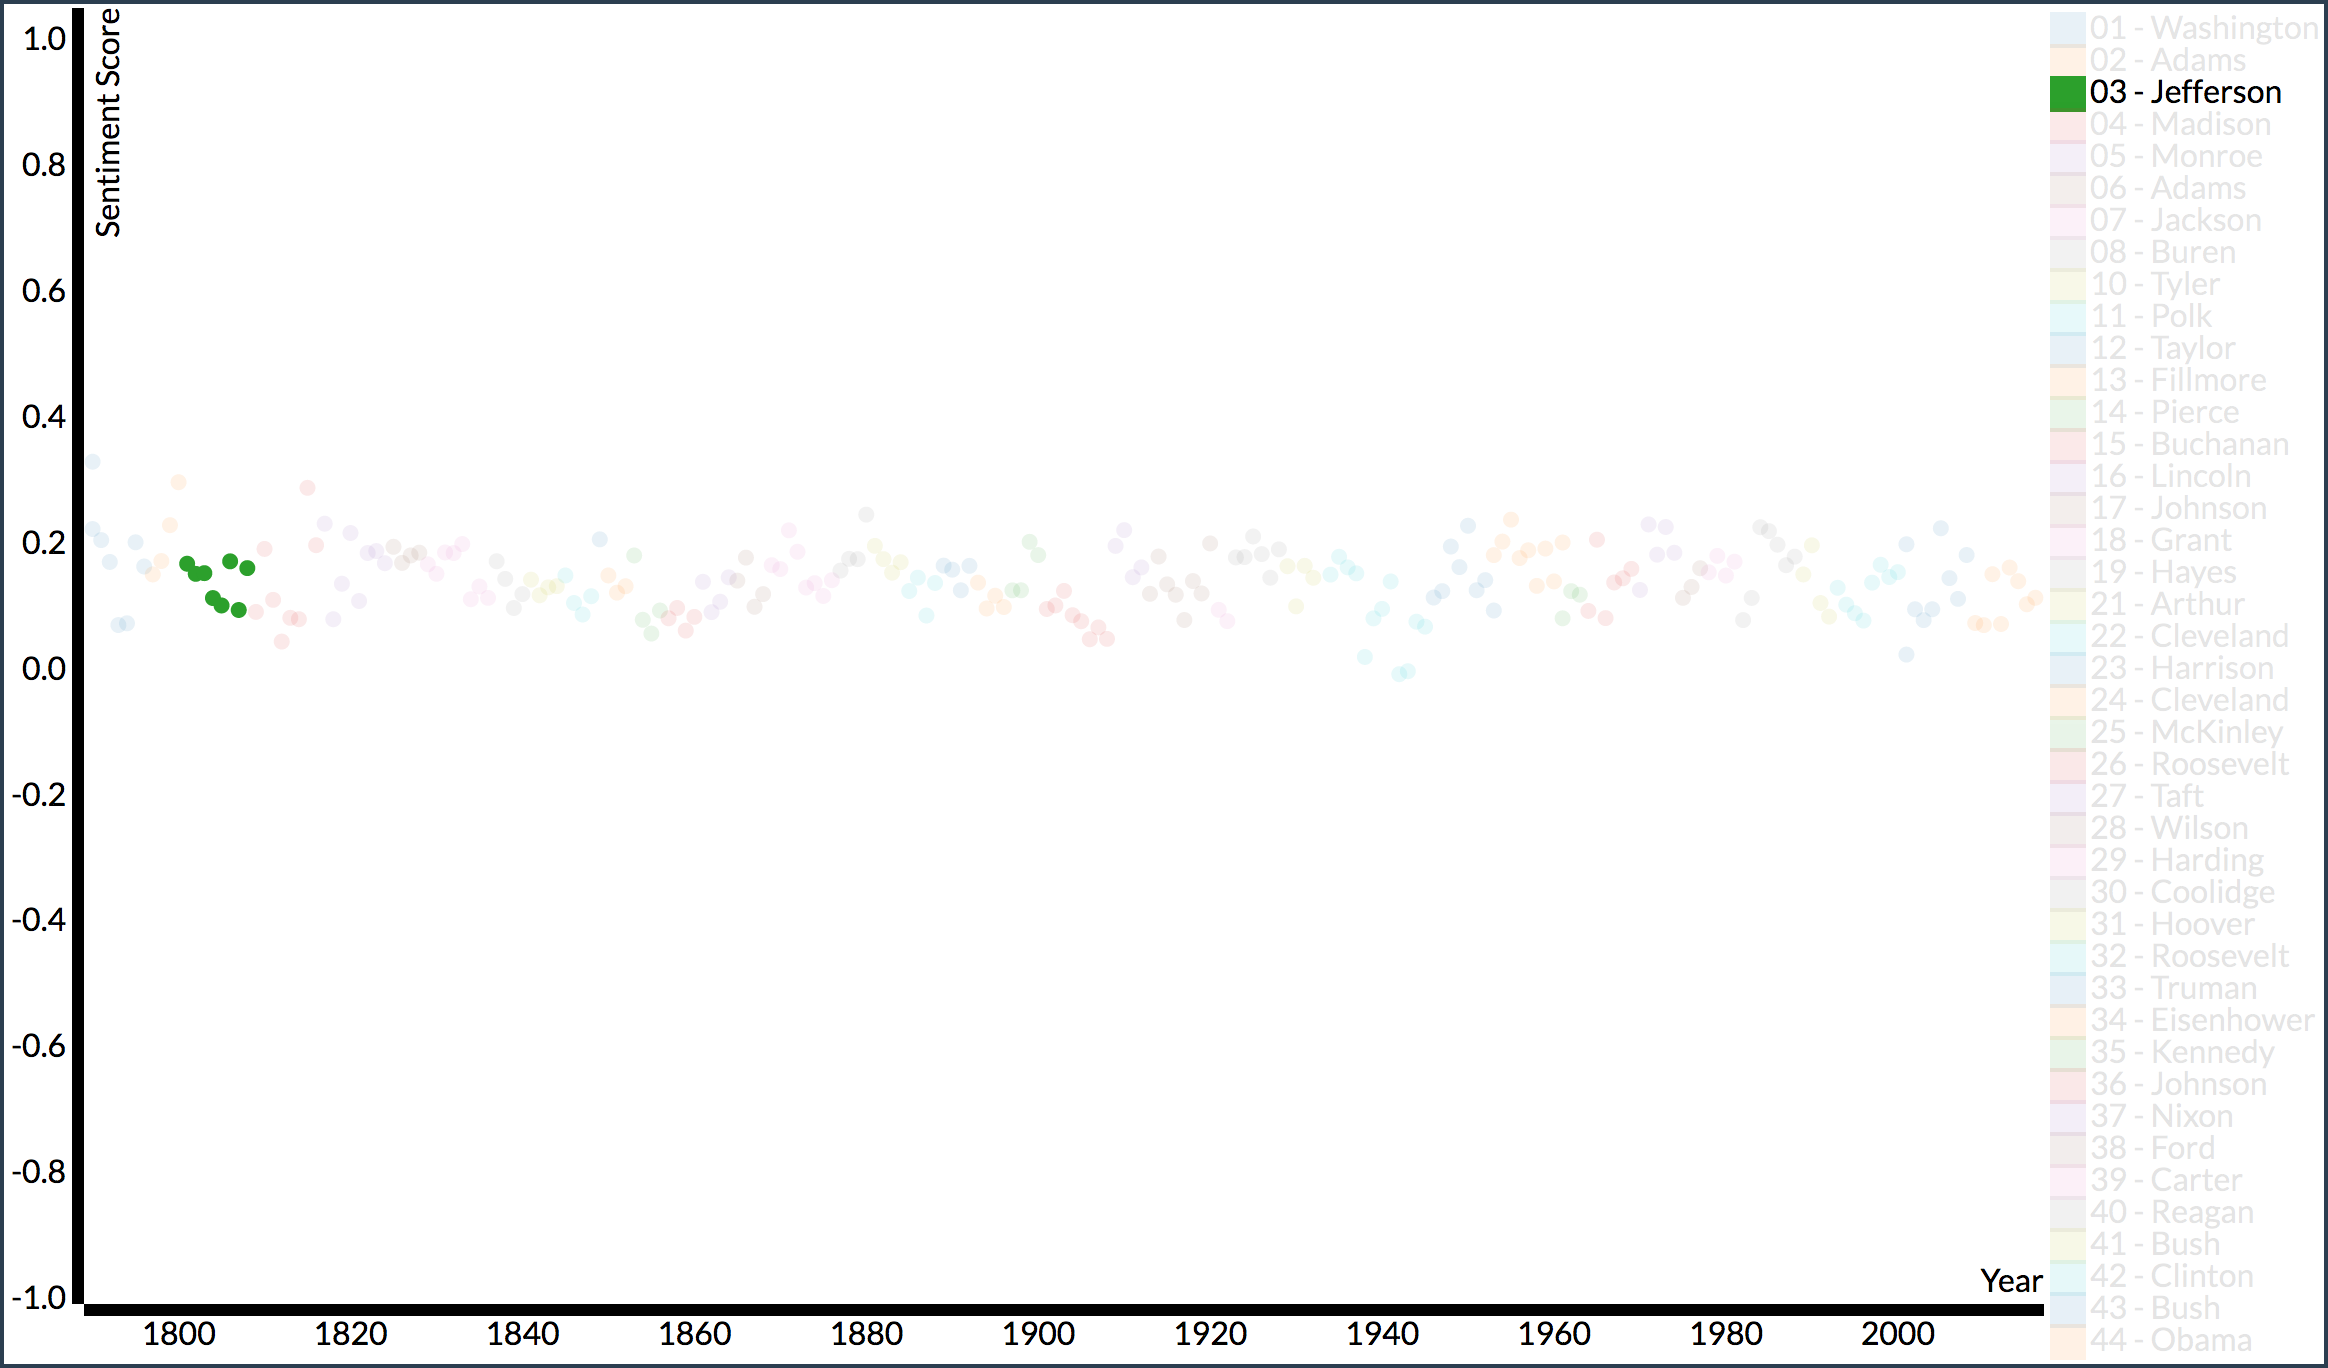
\includegraphics[width=\columnwidth]{Lineplothover.png}
  \caption{Line Plot showing the hover effect}
  \label{fig:lineplot2}
\end{figure}
If you hover over the president's name/color in the legend then it will highlight that president's points on the plot and fade out all the others as can be seen in Figure \ref{fig:lineplot2}.
If you hover over a specific point on the plot then you will see expanded information about the point itself, with the president's name, address date, and the exact sentiment score.
There is an additional plot with similar functionality on the next page but that instead color codes the presidents based on political party so that it is easier to compare tone and sentiment across party lines.

\subsection{Word Clouds}
\begin{figure}
  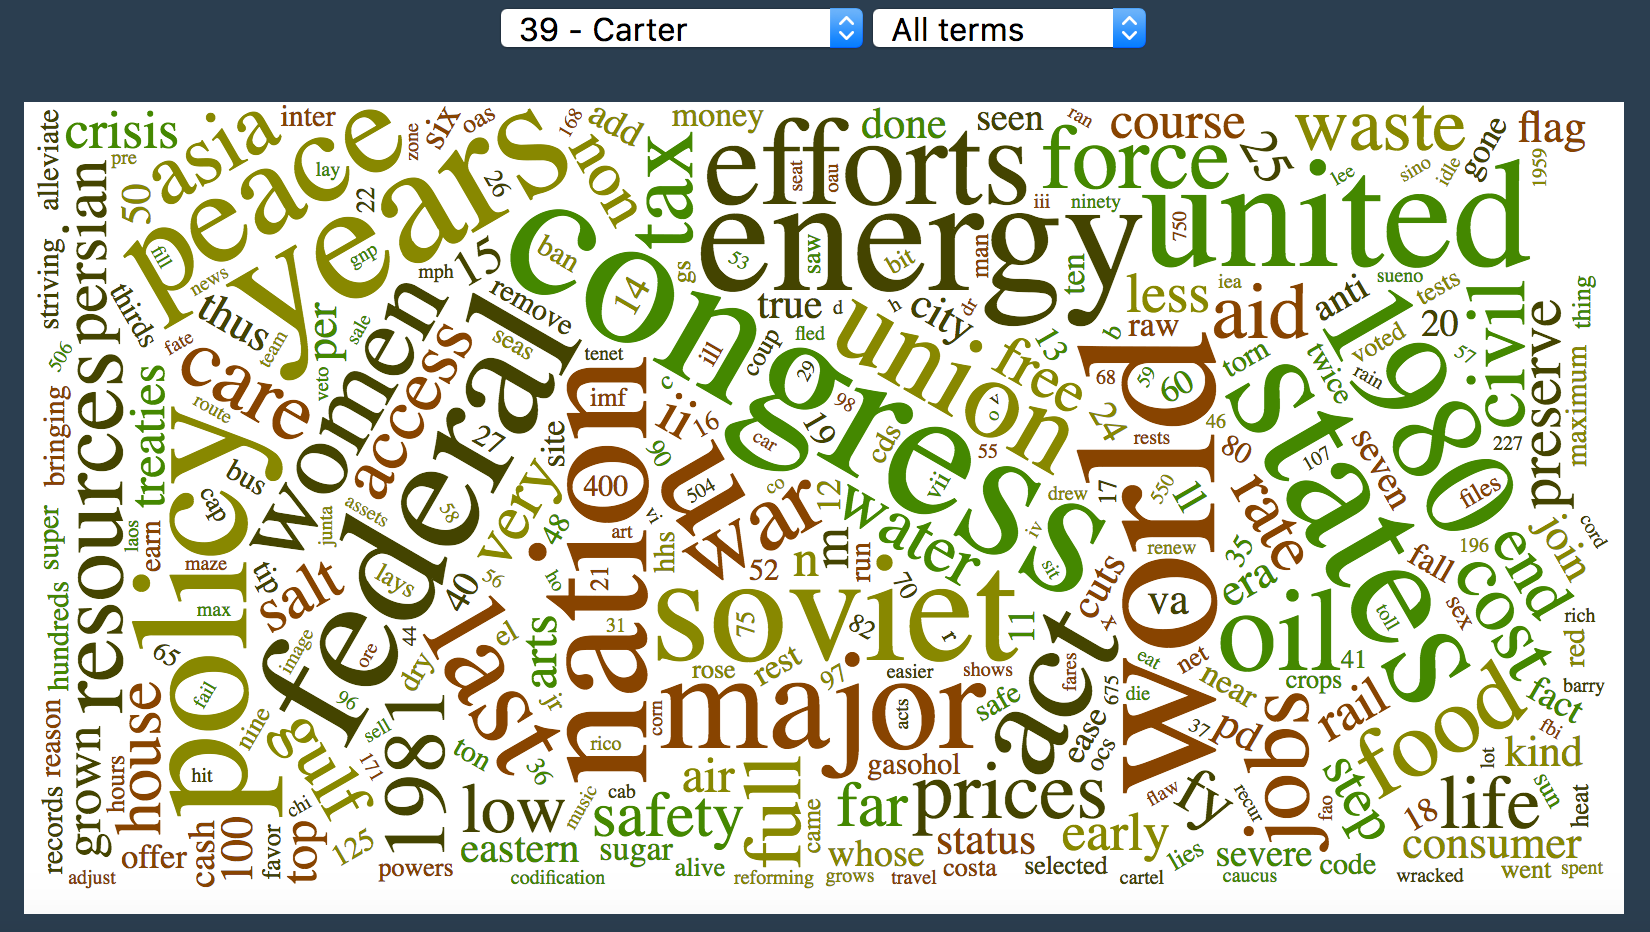
\includegraphics[width=\columnwidth]{Wordcloud.png}
  \caption{Example Word Cloud showing all terms for Jimmy Carter}
  \label{fig:wordcloud1}
\end{figure}
An additional visualization was added to the website that is popular among textual data and that visualization is a word cloud, an example of which can be seen in Figure \ref{fig:wordcloud1}.
A word cloud takes the most frequently used terms in a certain body of text and displays them in a collage format, with the size of each word indicating that terms relative frequency in the text.
Word clouds are often criticized when it comes to comparing actual frequencies of words since the relative size of each word is hard to distinguish, but here word clouds are used in more of a summarizing fashion, not as a means to compare any two speeches.
D3 was used here to create the wordclouds, as there is a D3 API called wordcloud that produces the word cloud using an array of JSON objects, with each object having a key that is the term and a value attribute that indicates the relative size of the word.
The API is finicky in some aspects of its implementation and requires the array to be sorted which was handled in the javascript before being fed into the API to produce each word cloud.
There is a slight delay in performance as the Word Clouds are rendered in real time as the respective SOTU addresses are loaded in to the API.
\begin{figure}
  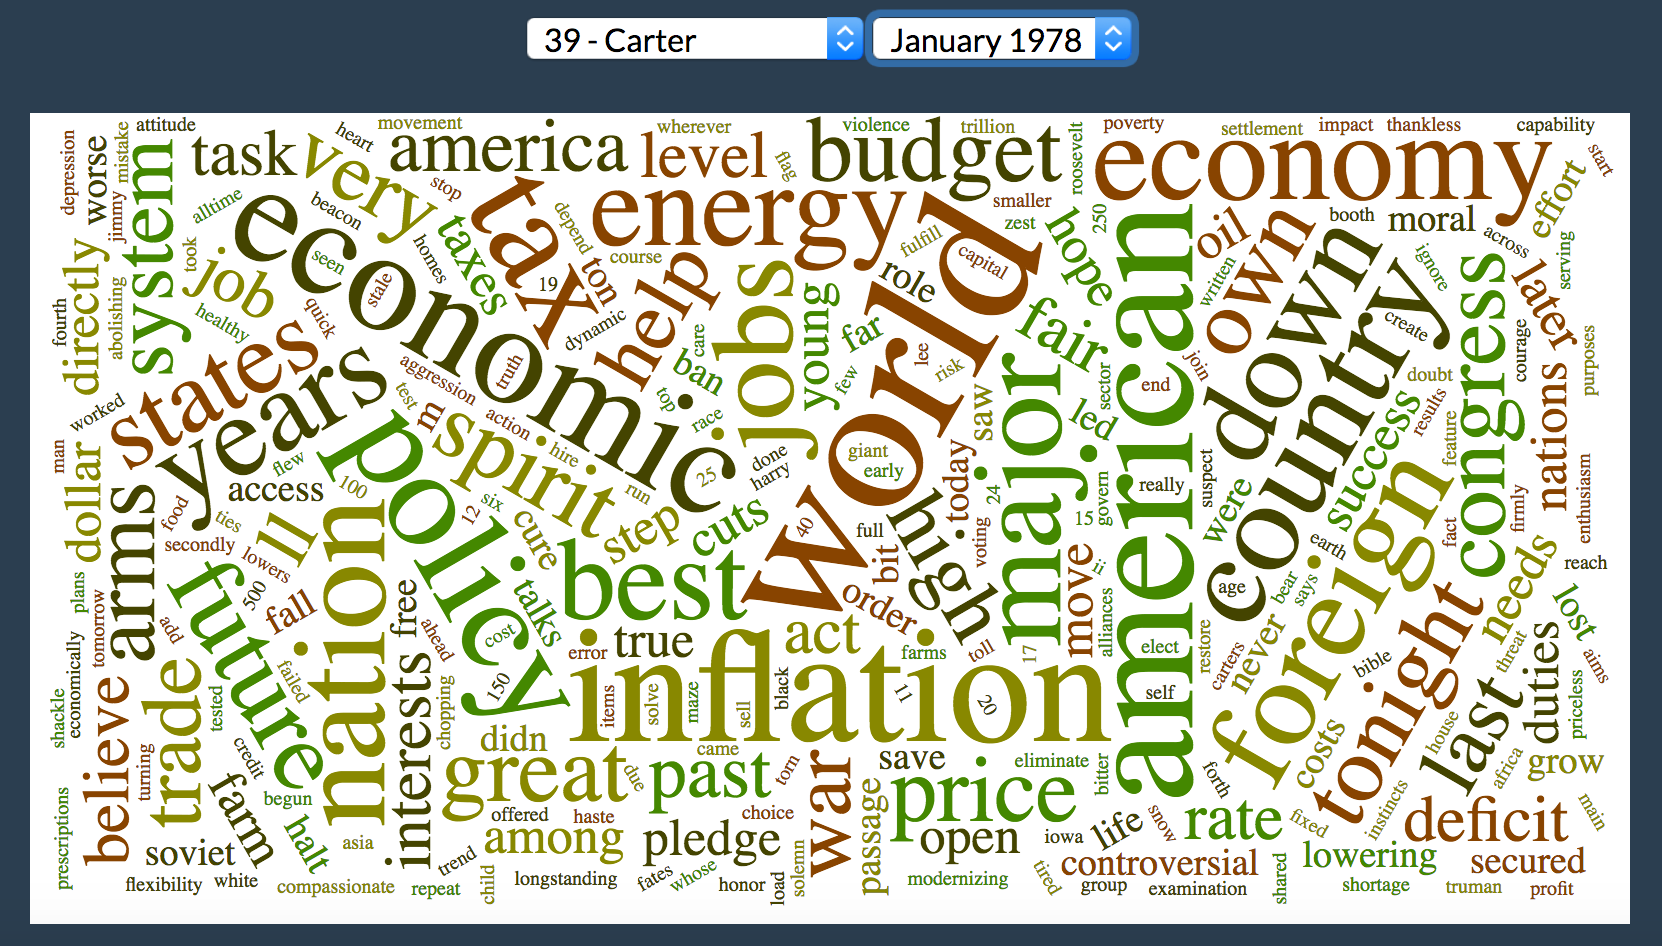
\includegraphics[width=\columnwidth]{Wordcloudterm.png}
  \caption{Example Word Cloud showing 1978 term for Jimmy Carter}
  \label{fig:wordcloud2}
\end{figure}
When a president is selected, the word clouds defaults to an overall word cloud for all of their terms and then another dropdown allowing you to choose a specific term to see that word cloud, as can be seen in Figure \ref{fig:wordcloud2}.

\section{Evaluation}
Validation is important in verifying the effectiveness of all algorithms and it is especially important when dealing with natural language data.
The two important validation steps here are to validate the effectiveness at which the sentiment score captured the overall tone of an address, and also verifying that the algorithm provides consistent results, which can be done using leave-one-out cross-validation.

\subsection{Validating Sentiment Analysis}
The effectiveness of a sentiment analysis relies heavily on the lexicon it is using to calculate sentiment score.
Here, the lexicon used is a widely-accepted and crowd-sourced effort to quantify tone in words and the closest one could get to an effective score with which to calculate these scores.
In order to validate the validity of the score for each address, the address with the highest sentiment score, the address with the lowest sentiment score, and an address from the middle were chosen and read manually and confirmed they belonged where they were.

\subsection{Leave-one-out Cross-validation}
Another validation method that is going to be used once the algorithm is improved is leave-one-out cross-validation.
In this method, each address is represented as a vector of 14 numbers, indicating the sentiment scores for each category as well as the overall score \cite{validation}.
Then, using these vectors, one of them is hidden, and the rest of the vectors are used to predict the values for the hidden vector.
This validation method ensures the algorithm is working properly and can properly predict a set of values using the existing data set.

\section{Conclusion}
In conclusion, there is still much to be said about the use of language and how people express their thoughts and feelings in speeches.
This research shows that there is a great deal of potential with this algorithm to achieve a deeper understanding of how presidents construct their speeches and how they inform the American people.
There is still much to be perfected in the ways of the algorithm and the effectiveness of his implementation but its usefulness has been shown.
It is easy to see the dips in tone over certain periods of turmoil and the potential usefulness for such a tool is great in analyzing political trends, and presidential speaking patterns.
The application for this research is specific but the lexicon used is very general and thus can be applied to many other corpora.

\bibliographystyle{natdin}
\bibliography{thesis}

\begin{acks}
Thank you so much to Dr. Wilkins for guiding me on this long journey and always being there when I need her. You are a true inspiration and have been so influential in my undergraduate career, and I'm so thankful for all your advice and help with this paper and this thesis.
\end{acks}

\end{document}
